\documentclass[a4paper,11pt,twoside]{report}
% KOMPILOWAĆ ZA POMOCĄ pdfLaTeXa, PRZEZ XeLaTeXa MOŻE NIE BYĆ POLSKICH ZNAKÓW

% -------------- Kodowanie znaków, język polski -------------

\usepackage[utf8]{inputenc}
\usepackage[MeX]{polski}
\usepackage[T1]{fontenc}
\usepackage[english,polish]{babel}


\usepackage{amsmath, amsfonts, amsthm, latexsym} % głównie symbole matematyczne, środowiska twierdzeń

\usepackage[final]{pdfpages} % inputowanie pdfa
%\usepackage[backend=bibtex, style=verbose-trad2]{biblatex}


% ---------------- Marginesy, akapity, interlinia ------------------

\usepackage[inner=20mm, outer=20mm, bindingoffset=10mm, top=25mm, bottom=25mm]{geometry}


\linespread{1.5}
\allowdisplaybreaks

\usepackage{indentfirst} % opcjonalnie; pierwszy akapit z wcięciem
\setlength{\parindent}{5mm}


%--------------------------- ŻYWA PAGINA ------------------------

\usepackage{fancyhdr}
\pagestyle{fancy}
\fancyhf{}
% numery stron: lewa do lewego, prawa do prawego 
\fancyfoot[LE,RO]{\thepage} 
% prawa pagina: zawartość \rightmark do lewego, wewnętrznego (marginesu) 
\fancyhead[LO]{\sc \nouppercase{\rightmark}}
% lewa pagina: zawartość \leftmark do prawego, wewnętrznego (marginesu) 
\fancyhead[RE]{\sc \leftmark}

\renewcommand{\chaptermark}[1]{
\markboth{\thechapter.\ #1}{}}

% kreski oddzielające paginy (górną i dolną):
\renewcommand{\headrulewidth}{0 pt} % 0 - nie ma, 0.5 - jest linia


\fancypagestyle{plain}{% to definiuje wygląd pierwszej strony nowego rozdziału - obecnie tylko numeracja
  \fancyhf{}%
  \fancyfoot[LE,RO]{\thepage}%
  
  \renewcommand{\headrulewidth}{0pt}% Line at the header invisible
  \renewcommand{\footrulewidth}{0.0pt}
}



% ---------------- Nagłówki rozdziałów ---------------------

\usepackage{titlesec}
\titleformat{\chapter}%[display]
  {\normalfont\Large \bfseries}
  {\thechapter.}{1ex}{\Large}

\titleformat{\section}
  {\normalfont\large\bfseries}
  {\thesection.}{1ex}{}
\titlespacing{\section}{0pt}{30pt}{20pt} 
%\titlespacing{\co}{akapit}{ile przed}{ile po} 
    
\titleformat{\subsection}
  {\normalfont \bfseries}
  {\thesubsection.}{1ex}{}


% ----------------------- Spis treści ---------------------------
\def\cleardoublepage{\clearpage\if@twoside
\ifodd\c@page\else\hbox{}\thispagestyle{empty}\newpage
\if@twocolumn\hbox{}\newpage\fi\fi\fi}


% kropki dla chapterów
\usepackage{etoolbox}
\makeatletter
\patchcmd{\l@chapter}
  {\hfil}
  {\leaders\hbox{\normalfont$\m@th\mkern \@dotsep mu\hbox{.}\mkern \@dotsep mu$}\hfill}
  {}{}
\makeatother

\usepackage{titletoc}
\makeatletter
\titlecontents{chapter}% <section-type>
  [0pt]% <left>
  {}% <above-code>
  {\bfseries \thecontentslabel.\quad}% <numbered-entry-format>
  {\bfseries}% <numberless-entry-format>
  {\bfseries\leaders\hbox{\normalfont$\m@th\mkern \@dotsep mu\hbox{.}\mkern \@dotsep mu$}\hfill\contentspage}% <filler-page-format>

\titlecontents{section}
  [1em]
  {}
  {\thecontentslabel.\quad}
  {}
  {\leaders\hbox{\normalfont$\m@th\mkern \@dotsep mu\hbox{.}\mkern \@dotsep mu$}\hfill\contentspage}

\titlecontents{subsection}
  [2em]
  {}
  {\thecontentslabel.\quad}
  {}
  {\leaders\hbox{\normalfont$\m@th\mkern \@dotsep mu\hbox{.}\mkern \@dotsep mu$}\hfill\contentspage}
\makeatother



% ---------------------- Spisy tabel i obrazków ----------------------

\renewcommand*{\thetable}{\arabic{chapter}.\arabic{table}}
\renewcommand*{\thefigure}{\arabic{chapter}.\arabic{figure}}
%\let\c@table\c@figure % jeśli włączone, numeruje tabele i obrazki razem


% --------------------- Definicje, twierdzenia etc. ---------------


\makeatletter
\newtheoremstyle{definition}%    % Name
{3ex}%                          % Space above
{3ex}%                          % Space below
{\upshape}%                      % Body font
{}%                              % Indent amount
{\bfseries}%                     % Theorem head font
{.}%                             % Punctuation after theorem head
{.5em}%                            % Space after theorem head, ' ', or \newline
{\thmname{#1}\thmnumber{ #2}\thmnote{ (#3)}}%  % Theorem head spec (can be left empty, meaning `normal')
\makeatother

% ----------------------------- POLSKI --------------------------------

\theoremstyle{definition}
\newtheorem{theorem}{Twierdzenie}[chapter]
\newtheorem{lemma}[theorem]{Lemat}
\newtheorem{example}[theorem]{Przykład}
\newtheorem{proposition}[theorem]{Stwierdzenie}
\newtheorem{corollary}[theorem]{Wniosek}
\newtheorem{definition}[theorem]{Definicja}
\newtheorem{remark}[theorem]{Uwaga}



% ----------------------------- Dowód -----------------------------

%\makeatletter
%\renewenvironment{proof}[1][\proofname]
%{\par
%  \vspace{-12pt}% remove the space after the theorem
%  \pushQED{\qed}%
%  \normalfont
%  \topsep0pt \partopsep0pt % no space before
%  \trivlist
%  \item[\hskip\labelsep
%        \sc
%    #1\@addpunct{:}]\ignorespaces
%}
%{%
%  \popQED\endtrivlist\@endpefalse
%  \addvspace{20pt} % some space after
%}
%
%\renewcommand{\qedhere}{\hfill \qedsymbol}
%\makeatother





% -------------------------- POCZĄTEK --------------------------


% --------------------- Ustawienia użytkownika ------------------

\newcommand{\tytul}{Tytuł pracy dyplomowej w języku polskim}
\renewcommand{\title}{English title}
\newcommand{\type}{inżyniers} % magisters, licencjac
\newcommand{\supervisor}{dr inż. Promotor X}



\begin{document}
\sloppy


\includepdf[pages=-]{strona_tytulowa-jeden-autor.pdf}


% ------------------ STRONA Z PODPISAMI AUTORA/AUTORÓW I PROMOTORA ------------------


\thispagestyle{empty}\newpage
\null

\vfill

\begin{center}
\begin{tabular}[t]{ccc}

............................................. & \hspace*{100pt} & .............................................\\
podpis promotora & \hspace*{100pt} & podpis autora


\end{tabular}
\end{center}



% ---------------------------- ABSTRAKTY -----------------------------
% W PRACY PO POLSKU, NAPIERW STRESZCZENIE PL, POTEM ABSTRACT EN

{
\begin{abstract}

\begin{center}
\tytul
\end{center}

Streszczam.

Lorem ipsum dolor sit amet, consetetur sadipscing elit, sed diam nonumyeirmod tempor invidunt ut labore et dolore magna aliquyam erat, sed diamvoluptua. At vero eos et accusam et justo duo dolores et ea rebum. Stet clita kasd gubergren, no sea takimata sanctus est Lorem ipsum dolor sit amet.\\

\noindent \textbf{Słowa kluczowe:} slowo1, slowo2, ...
\end{abstract}
}

\null\thispagestyle{empty}\newpage

{\selectlanguage{english}
\begin{abstract}

\begin{center}
\title
\end{center}

Lorem ipsum dolor sit amet, consetetur sadipscing elitr, sed diam nonumyeirmod tempor invidunt ut labore et dolore magna aliquyam erat, sed diamvoluptua. At vero eos et accusam et justo duo dolores et ea rebum. Stet clita kasd gubergren, no sea takimata sanctus est Lorem ipsum dolor sit amet.

Lorem ipsum dolor sit amet, consetetur sadipscing elitr, sed diam nonumyeirmod tempor invidunt ut labore et dolore magna aliquyam erat, sed diamvoluptua. At vero eos et accusam et justo duo dolores et ea rebum. Stet clita kasd gubergren, no sea takimata sanctus est Lorem ipsum dolor sit amet.\\

\noindent \textbf{Keywords:} keyword1, keyword2, ...
\end{abstract}
}


% --------------------- OŚWIADCZENIE -----------------------------------------


\null\thispagestyle{empty}\newpage

\null \hfill Warszawa, dnia ..................\\

\par\vspace{5cm}

\begin{center}
Oświadczenie
\end{center}

\indent Oświadczam, że pracę \type ką pod
tytułem ,,\tytul '', której promotorem jest \supervisor , wykonałam/wykonałem
samodzielnie, co poświadczam własnoręcznym podpisem.
\vspace{2cm}


\begin{flushright}
  \begin{minipage}{50mm}
    \begin{center}
      ..............................................

    \end{center}
  \end{minipage}
\end{flushright}

\thispagestyle{empty}
\newpage

\null\thispagestyle{empty}\newpage


% ------------------- 4. Spis treści ---------------------
\pagenumbering{gobble}
\tableofcontents
\thispagestyle{empty}

\newpage % JEŻELI SPIS TREŚCI MA PARZYSTĄ LICZBĘ STRON, ZAKOMENTOWAĆ
% ALBO JAK KTOŚ WOLI WTEDY DWIE STRONY ODSTĘPU, DODAĆ \null\newpage

% -------------- 5. ZASADNICZA CZĘŚĆ PRACY --------------------
\null\thispagestyle{empty}\newpage
\pagestyle{fancy}
\pagenumbering{arabic}
\setcounter{page}{11} % JEŻELI Z POWODU DUŻEJ ILOŚCI STRON W SPISIE TREŚCI SIĘ NIE ZGADZA, TRZEBA ZMODYFIKOWAĆ RĘCZNIE

\chapter*{Wstęp}
\markboth{}{Wstęp}
\addcontentsline{toc}{chapter}{Wstęp}

\chapter*{Opis problemu}

\section*{DNA}

DNA to molekuła składająca się z dwóch zwiniętych siebie nici tworzących podwójną helisę. DNA jest nośnikiem informacji genetycznej, przenoszącej instrukcje dotyczące rozwoju, funkcjonowania i reprodukcji wszystkich znanych organizmów żyjących i niektórych wirusów. Podstawowym składnikiem budującym DNA są nukleotydy. Każdy z nich zawiera jedną z czterech z zasad: adeninę, cytozynę, guaninę lub tyminę, często oznaczane pierwszą literą nazwy (odpowiednio A, C, G lub T). Sekwencja tych baz w DNA definiuje kod genetyczny. Kompletny kod genetyczny organizmu jest nazywany genomem. Długośc genomu znacznie róźni się pomiędzy gatunkami.


\begin{table}
\centering
\begin{tabular}{ll}
	Bakteria e. coli                                                                           & $\sim$4.6 miliona  \\
	\begin{tabular}[c]{@{}l@{}}Schizosaccharomyces pombe\\ (grzyb jednokomórkowy)\end{tabular} & $\sim$12.5 miliona \\
	\begin{tabular}[c]{@{}l@{}}Drosophila melanogaster\\ (muszka owocowa)\end{tabular}         & $\sim$170 milionów \\
	Oryza sativa (ryż)                                                                         & $\sim$470 milionów \\
	Canis familiaris (pies)                                                                    & $\sim$2.4 miliarda \\
	Homo sapiens (czlowiek)                                                                    & $\sim$2.9 miliarda
\end{tabular}
\caption{\label{}Liczba par zasad w genomach wybranych organizmów.}
\end{table}

\section*{Sekwencjonowanie DNA}

Sekwencjonowanie DNA to proces ropoznawania sekwencji DNA danego organizmu. Wczesne metody sekwencjonowania (np. metoda Sangera opracowana w 1977 r. \cite{sequencingTechnologies}) były zbyt kosztowne do powszechnych zastosowań, lecz metody dugiej i trzeciej generacji umożliwiły zbadanie DNA organizmów na szerszą skalę i wykorzystanie tej wiedzy w celach takich jak badanie odpornośći na nowotwory\cite{cancerImmunity} i przyczyn zachorwania na nie\cite{cancerNonCoding}, badanie historii adaptacji w procesie ewolucji człowieka \cite{adaptation}, medycyna spersonalizowana do kodu genetycznego człowieka \cite{personalizedMedicine}, badania prenatalne \cite{prenatal} i diagnostyka chorób o podłożu genetycznym\cite{diagnosis}.

Wynikiem sekwencjonowania jest fragment całego genomu. nazywanym odczytem(\textit{read}). Długośc odczytów jest zależna od użytej technologii - sekwencjonowanie technologią produkuje odczyty o długośći do 600 par zasad przy celności do 99.9\%, a przy użyciu technologii PacBio odczyty osiągają długośc nawet do 100 tysięcy par zasad przy celnośći 87\%. Odczyty są dopasowywane i łączone tak aby otrzymać cały genom(po angielsku ten proces jest nazywany \textit{genome assembly}).  Pomimo większej ilośći błędów w długich odczytach są one potrzebne do dopasowania regionów repetytywnych, czyli podsekwencji genomu występujących w nim wielokrotnie. Dla tego do składania genomu wykorzystuje się zarówno odczyty długie i krótkie.

\section*{Oxford Nanopore MinION}

Oxford Nanopore MinION to technologia sekwencjonowania dostępna publicznie od maja 2015 r. produkująca długie odczyty, nawet do 2 milionów par zasad. Wykorzystuje ona pory przez, które przepływa pojedyncza nić DNA. Wewnątrz nich mierzony jest sygnał elektryczny, które zmieniy się w zależności od tego, które nukleotydy znadują się wewnątrz poru. Na podstawie tego sygnału jest możliwe rozponanie sewkwencji DNA, nawet w trakcie procesu sekwencjonowania. Urządznie MinION jest bardzo przenośne (ma rozmiar zszywacza) i jego koszt jest znacznie mniejszy niż konkurencyjnych urządzeń. 

Proces rozpoznawania baz na podstawie sygnału elektrycznego wewnątrz poru nazywany jest basecallingiem. Jakość oprogramowania użytego do basecallingu (nazywanego basecallerem) ma znaczny wpływ na celność odczytów pochodzących z MinIONa.

\section*{Istniejące rozwiązania}

Oxford Nanopore Technologies (producent MinIONa) oferuje kilka basecallerów. Są to oficjalny basecaller Albacore, Guppy wykorzystujący procesory graficzne i Scrappie opisany przez producenta jako "demonstracja technologii". W przeszłości ONT oferowało również NanoNet oparty o sieci neuronowe, a także Metrichor działający w chmurze obliczeniowej.

Opublikowano również następujące basecallery z otwartym kodem źródłowym pochodzące od społecznośći badawczej.

DeepNano\cite{deepNano} wykonuje proces basecallingu w dwóch krokach. W pierwszym sygnał jest dzielony na fragmenty odpowiadjące k-merom. W drugim dwukierunkowa rekurencyjna sieć neuronowa wykorzystuje statystyki powstałych w pierwszym kroku fragmentów do przewidzenia k-meru odpowiadjącemu każdemu fragmentowi. 

BasecRAWller\cite{basecrawler} wykorzystuje dwie rekurencyjne sieci neuronowe. Pierwsza z nich przewiduje dla każdego kroku czasowego w sygnale wejściowym prawdopodobieństwo tego, że jest on granicą pomiędzy segmentom sygnału odpowiadjącego kolejnym nukleotydom. Druga mapuje w ten sposób powstałe segmenty na odpowiadające nim bazy.

Chiron\cite{chiron} tłumaczy sygnał elektryczny bezpośrednio na sekwencję DNA. Wykorzystuje on model oparty o sieci konwolucyjne, sieci rekurencyjne i dekodowanie CTC.
\chapter*{Opis rozwiązania}

\section*{Przygotowanie zbiorów danych danych}

W celu nauczenia i testowania sieci neuronowej przygotowane zostały 2 zbiory danych w postaci par \textit{wektor synału, odpowiadające mu nukleotydy}.
Pierwszy zbiór powstał z danych z sekwencjonowania genomu ludzkiego z lini komórkowej NA12878. Wykorzystano wyłącznie DNA pochodzące z chromosomu mitochondrialnego, na które składa się 5000 odczytów.
Dane pochodzące z sekwencjonowania metodą Nanopore pochodzą z repozytorium udostępnionego przez Whole Human Genome Sequencing Project\cite{nanoporeHuman},a genom referencyjny sekwencjonwany metodą Illumina pochodzi z The International Genome Sample Resource\cite{refGenome}. Aby uzyskać dane treningowe nie będące obciążone błędem innego \textit{basecallera} wykorzystano pakiet \textit{nanoraw}\cite{nanoraw}. Dokonuje on uliniowienia sygnału pochodzącego z sekwencjonowania technologią nanopore i genomu referencyjnego. W efekcie otrzymano podział sygnału na fragmenty, z których każdy odpowiada jednem z nukleotydów.

W celu poprawienia generalności rozwiązania do uczenia sieci wykorzystano również zbiór danych z sewkwencjonowania gatunków \textit{Escherichia virus Lambda} i \textit{Escherichia coli} składający się z 4000 odczytów \cite{chironData}. Uliniowienie z genomami referencyjnymi zostało wykonane przez autorów zbioru, w sposób analogiczny do opisanego powyżej.

\section*{Eksploracyjna analiza danych}

\section*{Reprezentacja i przygotowanie danych wejściowych}

\section{ReLU}

Funkcje aktywacji są stosowane w sieciach neuronowych w celu dodania nieliniowości do modelu. Są one stosowane do wyniku obliczeń warstw wewnątrz sieci. \textit{Recitified linear unit} czyli ReLU jest funkcją aktywacji daną wzorem
\[Relu(x) = max(0,x)\]

\section{\textit{Batch Normalization}}

\textit{Batch normalization} to metoda przyspieszająca uczenie sieci neuronowych, polegająca na normalizacji danych wejśćiowych do warstw ukrytych. Dzięki temu rozkład wartości aktywacji tych warstw pozostaje taki sam podczas całego procesu uczenia sieci. Wynik zastosowania \textit{Batch normalization } dla danych wejściowy $h$ jest danym wzorem:
\[BN(h, \lambda, \beta)=\beta+\lambda\frac{h-\hat{E}}{\sqrt{\hat{Var}(h)+\epsilon}}\]
gdzie $\lambda$ i $\beta$ są wagami nauczonymi przez sieć a $\epsilon$ to parametr regularyzujący.

\section*{Sieci konwolucyjne, ResNet}

Sieci konwolucyjne(splotowe) to klasa głębokich sieci neuronowych wykorzystujących operację konwolucji. Charakteryzują się one mniejszą ilością parametrów i lepszą umiejętnością uczenia się lokalnych cech danych wejśćiowych niż sieci w pełni połączone\cite{cnn} i dzięki temu znajdują zastosowanie w ekstrakcji cech w problemach, w których dane wejśćiowe są zależne od położenia lub czasu, takich jak rozpoznawanie obrazu \cite{vgg}, wideo\cite{cnnVideo} lub dźwięku\cite{cnnAudio}.

W przypadku sieci konwolucyjnych składających się z wielu warstw występuje problem zanikającego gradientu, co znacznie spowalnia lub uniemożliwa uczenia takich sieci\cite{difficulty}.
Architekturą, która próbuje rozwiązać tą trudność jest \textit{resNet}, osiągający jedne z najlepszych wyników w dziedzinie klasyfikacji obrazu. Sieci tego typu składają się z bloków zawierających połączenia omijające część warstw. Na wyjściu z każdego bloku znajduje się suma danych wejściowych i danych przetworzonych przez warstwy wenątrz bloku. Dzięki temu. sygnał nie zanika przed osiągnięciem dalszej części sieci. Umożliwiło to trenowanie sieci o większej liczbie warstw bez utraty celności predykcji.\cite{resnet}.

\begin{figure}[h!]
	\centering
	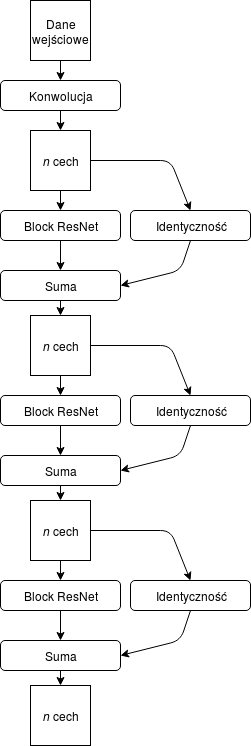
\includegraphics[scale=0.7]{resnet}
	\caption{Schemat połączeń w sieci ResNet składającej się z 3 bloków.}
\end{figure}

Ulepszona wersja tej architektury zawierająca mapowania identycznościowe została zaprezentowana w \cite{preResnet}. Autorzy propnują taką modyfikację sieci, aby dane wejściowe były dodawane do kolejnych warstw bez żadnych modyfikacji.We wcześniejszej wersji do danych wejśćiowych stosowano funkcje aktywacji i funkcje normalizujące. Zapobiega to zanikaniu gradientu nawet w sieciach składających się z tysiąca warstw. Dzięki temu można uniknąć efektu pogarszania się jakości predykcji wraz ze zwiekszaniem ilości warstw w sieci powyżej określonej liczby.

\begin{figure}[h!]
	\centering
	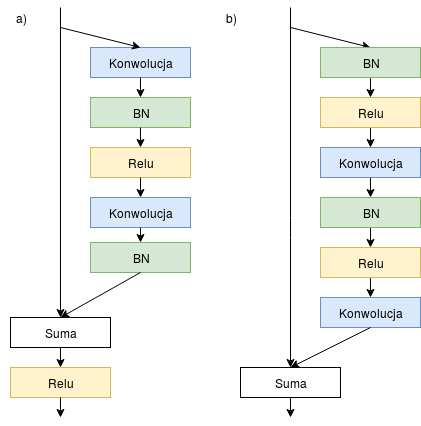
\includegraphics{resnetBlock}
	\caption{Konstrukcja bloku użytego w sieci resNet w wersji a) orygninalnej i b) z mapowaniem identycznościowym}
\end{figure}

\section{DenseNet}

W architekturze DenseNet, będącej rozwnięciem idei wykorzystanych w ResNet, każda z warstw przekazuje do dalszej części sieci skontatenowane wyniki obliczeń wykonanych przez siebie i każdą z poprzednich warstw. Na wyjściu z sieci znajdują sie cechy obliczone, przez każdą z warstw w sieci - wynikami kolejnych warstw są cechy danych wejśćiowych coraz wyższego rzędu. Dzięki temu wszystkie warstwy w sieci podlegają nadzorowi, podobnie jak w sieciach DSN(Deeply-Supervised Nets)\cite{DSN}. Wykorzystanie cech obliczonych w począktwych warstwach w dalszej części sieci, umożliwia zastosowanie modeli o mniejszej liczbie parametrów. Klasyfikacja jest dokonywana na podstawie cech niskiego i wysokiego rzędu. Dzięki temu sieci typu DenseNet osiągają lepszą precyzję klasyfikacji, niż sieci typu ResNet, mimo zastosowania mniej złożonego modelu\cite{denseNet}. 

\begin{figure}[h!]
	\centering
	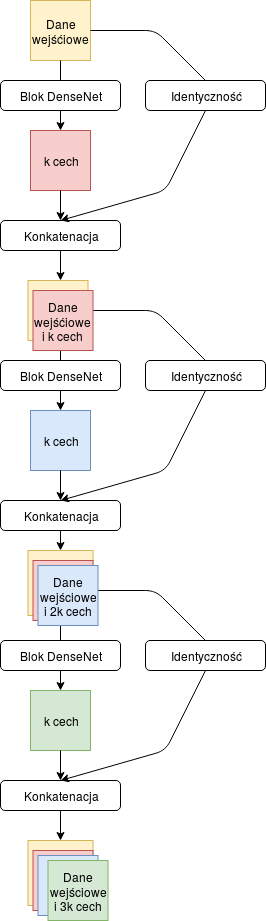
\includegraphics[scale=0.7]{densenet}
	\caption{Schemat połączeń w sieci DenseNet składającej się z 3 bloków.}
\end{figure}

\section*{Sieci w pełni konwolucyjne}

Sieci w pełni konwolucyjne to rodzaj sieci składających się wyłącznie z warstw konwolucyjnych, które mogą być zastosowane w problemach w których rozmiar danych wyjściowych, jest zależny od rozmiaru danych wejściowych, takich jak segmentacja obrazu\cite{segmentation} czy modelowanie sekwencji np. dzwięku i tekstu \cite{sequenceModelling}. Wykorzystują one fakt, że każdy neuron w sieci przetwarza tylko dane wejściowe znajdującym się w w jego otoczeniu, którego rozmiar zależy od rozmiaru filtrów w poprzedzających go warstwach. Zatem w sieci składające sie wyłącznie z warstw konwolucyjnych, liczba neuronów w ostatniej warstwie jest zależna od rozmiaru danych wejśćiowych i każdy z tych neuronów odpowiada, pewnemu elementowi z danych wejśćiowych, np. krokowi czasowemu lub pikselowi w obrazie\cite{fcn}.

Czasowe sieci konwolucyjne(\textit{temporal convolutional networks}) to sieci w pełni konwolucyjne dostosowane do problemów, w których dane wejściowe zależą od czasu. Stosuje się w nich konwolucje przyczynowe(causal convolutions), czyli takie, w których predykcja dla kroku czasowego \textit{t} zależy tylko od danych wejśćiowych dla kroku czasowego \textit{t} i wcześniejszych. Aby zwiększyć pole recepcyjne wykorzystano konwolucje rozszerzone (\textit{dilated convolutions}). Polega ona na wykorzystaniu wartośći oddalonych o \textit{d} kroków czasowych przy obliczaniu wartości filtra, gdzie \textit{d} jest parameterem. Paramter ten jest zwiększany wykładniczo w kolejnych warstwach, co pozwala na wykorzystanie w predykcji danych dla oddalonych kroków czasowych.

\begin{figure}[h!]
	\centering
	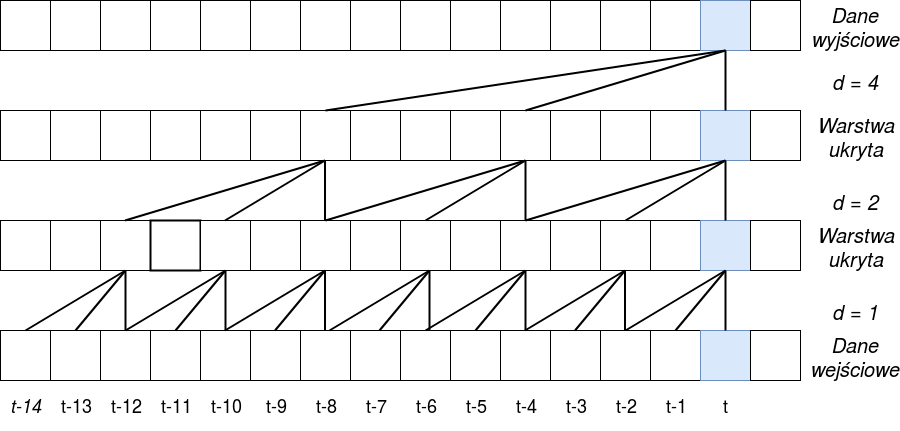
\includegraphics[scale=0.5]{tcn}
	\caption{Schemat przedstawiający połaczenia w sieci używającej konwolucji czasowych i przyczynowych.}
\end{figure}

Czasowe sieci konwolucyjne znalazły zastosowanie w problemach, w których dane wejśćiowe są zależne od czasu np. tłumaczenie maszynowe\cite{fcnTranslation} i synteza dźwięku. Innym typem sieci znajdujących zastosowanie w tej klasie problemów są sieci LSTM\cite{lstm}, lecz zademonstrowano, że sieci w pełni konwolucyjne są w stanie osiągać lepsze wyniki w wielu problemach, mimo mniejszego zużycia pamięci i krótszego czasu potrzebnego do wykonania obliczeń \cite{sequenceModelling}.

\section*{WaveNet}

Wavenet to głęboka sieć neuronowa wykorzystana oryginalnie do syntezy mowy\cite{wavenet}. Wykorzystano w niej konwolucje rozszerzone i przyczynowe tak jak w czasowych sieciach konwolucyjnych. Do wyniku obliczeń każdej z warstw konwolucyjnych stosuje sie funkcję sigmoidalną i tangens hiperboliczny. Do dalszej części sieci przekazywany iloczyn wyników zastosowania tych funkcji. Podobna operacja jest wykonywana w sieciach LSTM \cite{lstm}, i tak ja tam ma za zadanie znormalizowanie cech i wybranie, które z nich mają przekazane do dalszej części sieci. Dodatkowo wykorzystano połączenia rezydualne podobne do tych w sieci ResNet\cite{resnet}, a klasyfikacja jest dokonywana na podstawie sumy cech obliczonej przez każdą z warstw.

\begin{figure}[h!]
	\centering
	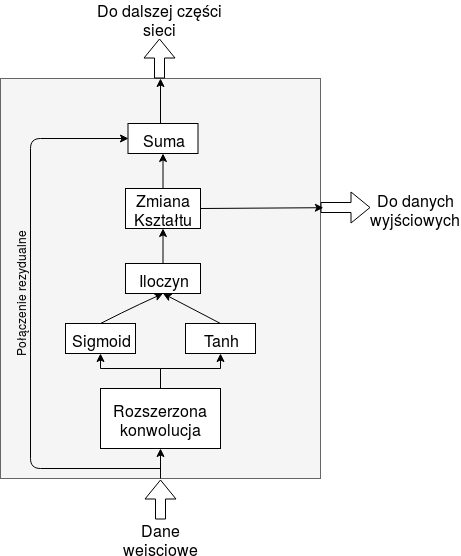
\includegraphics[scale=0.7]{wavenet_block}
	\caption{Blok sieci Waveneta. Sieć składa się z pewnej liczby takich bloków połączonych w serii.}
\end{figure}

Sieci Wavenet udało się wygenerować mowę bardzo podobną do ludzkiej\cite{wavenet}, znalazła ona również zastosowanie w problemach rozpoznawania mowy, redukcji hałasu i generowania muzyki\cite{wavenetReview}.

\section*{Dekodowanie CTC}

Zarówno sieci konwolucyjne jak i sieci LSTM mogą przyjmować dane wejściowe różnych rozmiarów, ale rozmiar danych wyjściowych jest funkcją rozmiaru danych wejściowych. W celu zbudowania modelu, który dla danych o określonym rozmiarze może zwracać sekwencje różnych długości stosuje sie dekodowanie CTC(\textit{Connectionist Temporal Classification})\cite{ctc}. Dekoder CTC przyjmuje na wejśćiu macierz o rozmiarze \textit{(rozmiar alfabetu wyjśćiowego + 1, długość sekwencji wejśćiowej)}. Element macierzy na pozycji  \textit{(n, t)} opisuje prawdopodbieńśtwo, że krok czasowy \textit{t} danych wejśćiowych odpowiada \textit{n}-temu elementowi alfabetu wyjśćiowego. Ostatni wiersz macierzy odpowiada prawdopobieństwu wystąpienia dodatkowego symbolu - znaku pustego odpowiadającemu granicom pomiędzy kolejnymi znakami w ciągu wyjściowym. 

Sekwencje są enkodowane w tej macierzy przez ścieżki, które powstają poprzez wybranie jednego znaku dla każdego kroku czasowego. Ścieżka zostaje zamieniona na sekwencję wyjśćiową poprzez połączenie w nieprzerwanych podciągów składających się z jednego znaku w pojedyńczy symbol(AAAAAA -> A), a następnie usunięcie znaków pustych. Zatem sekwencje wyjśćiowe mogą być krótsze niż sekwencje wejściowe i mogą zawierać te same znaki na sąsiadujących pozycjach, w przypadku gdy w ścieżce znajduje się pomiędzy nimi znak pusty. Prawdopodbieńśtwo śćieżki jest zdefiniowane prez iloczyn prawdopodbieństw wybranych znaków dla każdego kroku czasowego.

\begin{figure}[h!]
	\centering
	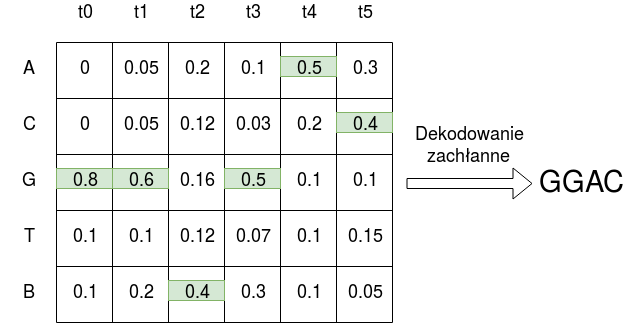
\includegraphics[scale=0.8]{ctc_array}
	\caption{Przykład dekodowania CTC dla alfabetu wyjśćioweg {A,C,G,T} i sekwencji wejściowej długośći 6.}
\end{figure}

Prawdopodobieństwo sekwencji wyjściowej to suma prawdopodobieństw wszystkich ścieżek, które mogą zostać zamienione na tą sekwencję. Znalezienie optymalnego rozwiązania problemu wybrania ścieżki o największym prawdopodbieństwie jest zbyt skomplinowane obliczeniowo, więc zamiast tego stosuje się alogrytm zachłanny, który wybiera dla każdego kroku czasowego znak o największym prawdopodobieństwie lub algorytm \textit{beam search}, który dla każdego kolejnego kroku czasowego zapamiętuje określoną liczbę najlepszych kandydatów. W przypadku dokonywania predykcji przez model jako sekwencja wyjśćiowa wybierana jest ta znaleziona przez jeden z tych algorytmów.

Funkcja straty dla dekodowania CTC zdefiniowana jest jako
\[-\ln{(p(x|z))}\]
gdzie $p(x|z)$ to prawdopobieńśtwo prawdziwej sekwencji dla danej macierzy prawdopodobieństw dla kroków czasowych.


\section*{Architektury przetestowanych sieci neuronowych}

\section*{Składanie odczytów}

\chapter*{Analiza wyników}

\section*{Zbiory danych}

\section*{Szczegóły techniczne implementacji}

\section*{Ewaluacja testowanych architektur sieci}

\section*{Porównanie najlepszego z przygotowanych rozwiązań z istniejącymi rozwiązaniami}

\section*{Testy wydajności}

\chapter{Wnioski}
% -------------------- 6. Bibliografia -----------------------
% Bibliografia leksykograficznie wg nazwisk autorów
% Dla ambitnych - można skorzystać z BibTeX-a

\begin{thebibliography}{20}%jak ktoś ma więcej książek, to niech wpisze większą liczbę
% \bibitem[numerek]{referencja} Autor, \emph{Tytuł}, Wydawnictwo, rok, strony
% cytowanie: \cite{referencja1, referencja 2,...}
\bibitem{genome}James Fraser, Iain Williamson, Wendy A. Bickmore,  Josée Dostie, An Overview of Genome Organization and How We Got There: from FISH to Hi-C
\bibitem{cancerImmunity}Finotello, F., Rieder, D., Hackl, H. et al. Next-generation computational tools for interrogating cancer immunity. Nat Rev Genet 20, 724–746 (2019) doi:10.1038/s41576-019-0166-7
\bibitem{cancerNonCoding}Khurana, E., Fu, Y., Chakravarty, D. et al. Role of non-coding sequence variants in cancer. Nat Rev Genet 17, 93–108 (2016) doi:10.1038/nrg.2015.17
\bibitem{adaptation} Marciniak, S., Perry, G. Harnessing ancient genomes to study the history of human adaptation. Nat Rev Genet 18, 659–674 (2017) doi:10.1038/nrg.2017.65
\bibitem{personalizedMedicine} Ashley, E. Towards precision medicine. Nat Rev Genet 17, 507–522 (2016) doi:10.1038/nrg.2016.86
\bibitem{prenatal} Chiu, R. W. et al. Noninvasive prenatal diagnosis of fetal chromosomal aneuploidy by massively parallel genomic sequencing of DNA in maternal plasma. Proc. Natl Acad. Sci. USA105, 20458–20463 (2008)
\bibitem{diagnosis} Choi, M. et al. Genetic diagnosis by whole exome capture and massively parallel DNA sequencing. Proc. Natl Acad. Sci. USA106, 19096–19101 (2009).
\bibitem{sequencingComparison} Liu L, Li Y, Li S, Hu N, He Y, Pong R, Lin D, Lu L, Law M (1 January 2012). "Comparison of Next-Generation Sequencing Systems". Journal of Biomedicine and Biotechnology. 2012: 251364. doi:10.1155/2012/251364.
\bibitem{sequencing} Jay Shendure Shankar Balasubramanian, George M. Church, Walter Gilbert, Jane Rogers, Jeffery A. Schloss, Robert h. Waterston DNA sequencing at 40: past, present and future
\bibitem{sequencingTechnologies} James M.Heather, Benjamin Chain The sequence of sequencers: The history of sequencing DNA
\bibitem{refGenome} Susan Fairley, Ernesto Lowy-Gallego, Emily Perry, Paul Flicek, The International Genome Sample Resource (IGSR) collection of open human genomic variation resources, Nucleic Acids Research.
\bibitem{nanoporeHuman} Miten Jain, Sergey Koren, Karen H Miga, Josh Quick, Arthur C Rand, Thomas A Sasani, John R Tyson, Andrew D Beggs, Alexander T Dilthey, Ian T Fiddes, Sunir Malla, Hannah Marriott, Tom Nieto, Justin O'Grady, Hugh E Olsen, Brent S Pedersen, Arang Rhie, Hollian Richardson, Aaron R Quinlan, Terrance P Snutch, Louise Tee, Benedict Paten, Adam M Phillippy, Jared T Simpson, Nicholas J Loman \& Matthew Loose. Nanopore sequencing and assembly of a human genome with ultra-long reads. Nature Biotechnology
\bibitem{deepNano}Boza, V., Brejova, B. \& Vinar, T. Deepnano: Deep recurrent neural networks for base calling in minion nanopore reads.PloS one12, e0178751 (2017).
\bibitem{basecrawler}Stoiber, M. \& Brown, J. Basecrawller: Streaming nanopore basecalling directly from raw signal.bioRxiv133058 (2017).
\bibitem{chiron} Haotian Teng, Minh Duc Cao, Michael B Hall, Tania Duarte, Sheng Wang, Lachlan J M Coin, Chiron: translating nanopore raw signal directly into nucleotide sequence using deep learning, GigaScience, Volume 7, Issue 5, May 2018, giy037, https://doi.org/10.1093/gigascience/giy037
\bibitem{nanoraw}Stoiber, M.H. et al. De novo Identification of DNA Modifications Enabled by Genome-Guided Nanopore Signal Processing. bioRxiv (2016).
\bibitem{chironData} Teng H; Cao MD; Hall MB; Duarte T; Wang S; Coin LJM (2018): Supporting data for "Chiron: Translating nanopore raw signal directly into nucleotide sequence using deep learning" GigaScience Database.
\bibitem{resnet} K. He, X. Zhang, S. Ren and J. Sun, “Deep Residual Learning for Image Recognition,” in CVPR, 2016.
\bibitem{preResnet}K. He, X. Zhang, S. Ren, and J. Sun. Identity Mappings in Deep Residual Networks. arXiv preprint arXiv:1603.05027v3,2016.
\bibitem{cnn}Yann LeCunn, Leon Bottou, Yoshua Bengio, Patrick Haffner, Gradient-Based Learning Applied to Document Recognition, 1998
\bibitem{vgg}Very Deep Convolutional Networks for Large-Scale Image Recognition Karen Simonyan, Andrew Zisserman
\bibitem{cnnVideo} Exploiting Image-trained CNN Architectures for Unconstrained Video Classification Shengxin Zha, Florian Luisier, Walter Andrews, Nitish Srivastava, Ruslan Salakhutdinov
\bibitem{cnnAudio} Environmental Sound Classification With Convolutional Neural Networks Karol J. Piczak
\bibitem{difficulty}Understanding the difficulty of training deep feedforward neural networks Xavier Glorot, Yoshua Bengio
\bibitem{segmentation} Recent progress in semantic image segmentation Xiaolong Liu, Zhidong Deng, Yuhan Yang
\bibitem{sequenceModelling} An Empirical Evaluation of Generic Convolutional and Recurrent Networks for Sequence Modeling Shaojie Bai, J. Zico Kolter, Vladlen Koltun
\bibitem{bn}Sergey Ioffe, Christian Szegedy Batch Normalization: Accelerating Deep Network Training by Reducing Internal Covariate Shift https://arxiv.org/abs/1502.03167
\bibitem{fcn}Fully Convolutional Networks for Semantic Segmentation Jonathan Long, Evan Shelhamer, Trevor Darrell
\bibitem{DSN}Deeply-Supervised Nets Chen-Yu Lee, Saining Xie, Patrick Gallagher, Zhengyou Zhang, Zhuowen Tu
\bibitem{denseNet}Densely Connected Convolutional Networks Gao Huang, Zhuang Liu, Laurens van der Maaten, Kilian Q. Weinberger
\bibitem{fcnTranslation}Pervasive Attention: 2D Convolutional Neural Networks for Sequence-to-Sequence Prediction Maha Elbayad, Laurent Besacier, Jakob Verbeek
\bibitem{lstm} Sepp Hochreiter; Jürgen Schmidhuber Long short-term memory. Neural Computation
\bibitem{tcn} Nal Kalchbrenner  Lasse Espeholt  Karen Simonyan  Aaron van den Oord  Alex Graves  Koray Kavukcuoglu Neural Machine Translation in Linear Time
\bibitem{wavenet}Aaron van den Oord, Sander Dieleman, Heiga Zen, Karen Simonyan, Oriol Vinyals, Alex Graves, Nal Kalchbrenner, Andrew Senior, Koray Kavukcuoglu WaveNet: A Generative Model for Raw Audio
\bibitem{wavenetReview} Boilard, Jonathan \& Gournay, Philippe \& Lefebvre, R.. (2019). A Literature Review of WaveNet: Theory, Application and Optimization. 
\bibitem{ctc}Alex Graves, Santiago Fernandez, Faustino Gomez, Jurgen Schmidhuber, Connectionist Temporal Classification: Labelling Unsegmented Sequence Data with Recurrent Neural Networks
\end{thebibliography}

\thispagestyle{empty}
\pagenumbering{gobble}



% --- 7. Wykaz symboli i skrótów - jeśli nie ma, zakomentować
\chapter*{Wykaz symboli i skrótów}

\begin{tabular}{cl}
nzw. & nadzwyczajny \\
* & operator gwiazdka \\
$\widetilde{}$ & tylda
\end{tabular}
\\
Jak nie występują, usunąć.
\thispagestyle{empty}


% ----- 8. Spis rysunków - jeśli nie ma, zakomentować --------
\listoffigures
\thispagestyle{empty}
Jak nie występują, usunąć.


% ------------ 9. Spis tabel - jak wyżej ------------------
\renewcommand{\listtablename}{Spis tabel}
\listoftables
\thispagestyle{empty}
Jak nie występują, usunąć.


% 10. Spis załączników - jak nie ma załączników, to zakomentować lub usunąć

\chapter*{Spis załączników}
\begin{enumerate}
\item Załącznik 1
\item Załącznik 2
\item Jak nie występują, usunąć rozdział.
\end{enumerate}
\thispagestyle{empty}


\end{document}
